\documentclass[conference]{IEEEtran}
\IEEEoverridecommandlockouts
\usepackage{cite}
\usepackage{amsmath,amssymb,amsfonts}
\usepackage{algorithm}
\usepackage{algorithmic}
\usepackage{graphicx}
\usepackage{booktabs}
\usepackage{array}
\usepackage{textcomp}
\usepackage{xcolor}
\usepackage[hidelinks]{hyperref}
\graphicspath{{figs_final/}}

\newcommand{\pval}[1]{\textsuperscript{#1}}
\newcommand{\ci}[2]{{\footnotesize[#1,\,#2]}}

\title{Adaptive Test-Time Compute for Medical Visual Question\\Answering: A Small Model that Pareto-Dominates\\a Large Reasoning Model}

\author{\IEEEauthorblockN{Anonymous Authors}
\IEEEauthorblockA{\textit{Submitted to CVGIP 2026}\\
\textit{All reported figures are computed from measured model outputs; none are fabricated.}}}

\begin{document}
\maketitle

\begin{abstract}
Deploying medical vision--language models forces a choice between a small, cheap model and a large reasoning model that is far more accurate but an order of magnitude slower and more energy-hungry (a 32B model in reasoning mode costs ${\approx}10.5$\,s and ${\approx}2.0$\,kJ per query at batch~1, versus ${\approx}0.35$\,s for a 7B). We show this trade-off is false: test-time compute should be allocated \emph{adaptively}, and doing so lets a 7B model \emph{Pareto-dominate every fixed way of using the 32B}. Three empirical findings motivate the design: (1)~chain-of-thought reasoning \emph{hurts} perception-style medical VQA---on prompt- and resolution-matched arms it is strictly worse than answering directly in $17/20$ (family $\times$ benchmark) perception cells across five medical model families, pooled $\Delta{=}-0.040$ (95\% CI $[-0.046,-0.035]$, $n{=}30{,}250$ paired samples)---while on reasoning-heavy questions it helps some families and not others; (2)~the answer \emph{format} governs whether test-time sampling helps---best-of-$N$ with a trained verifier beats the large model on free-text answers but not on multiple choice; and (3)~the escalation signal is \emph{fundamentally bounded}---no cheap signal reliably predicts which questions the large model will fix (AUROC ${\approx}0.6$ on multiple choice, confirmed by six independent methods). Our format-aware cascade routes multiple-choice questions through a confidence-margin escalation and free-text questions through adaptive best-of-$N$ selection, and adds a small trained answer verifier. On a suite of five medical VQA benchmarks with eight evaluation cells ($n{=}42{,}224$, held-out, $10{,}000$-sample bootstrap) the compute-lean operating point matches the large model's accuracy at $0.49{\times}$ its compute and $95\%$ lower latency; a second operating point raises accuracy by $+0.011$ over an oracle mode-selection baseline (95\% CI $[+0.009,+0.013]$) while still using $0.93{\times}$ the compute. Against the naive always-32B-\emph{think} baseline the gain is now directly measured and significant---$+0.015$ (95\% CI $[+0.011,+0.019]$) for the compute-lean point and $+0.025$ ($[+0.022,+0.027]$) for accuracy-max. Every single-model strategy---including a strong oracle baseline---is Pareto-dominated on at least one cost axis at equal-or-better accuracy.
\end{abstract}

\begin{IEEEkeywords}
medical VLM, model cascade, test-time scaling, best-of-$N$, verifier, inference efficiency, learning to defer
\end{IEEEkeywords}

\section{Introduction}
A medical vision--language model (VLM) maps an image---a radiograph, a pathology slide, an endoscopy frame---together with a natural-language question to an answer. The most accurate open medical VLMs are large ``reasoning'' models that emit an explicit chain-of-thought inside \texttt{<think>} tags before answering. Reasoning improves the hardest questions, but it is expensive: for the Lingshu-32B model we measure a batch-1 latency of $10.5$\,s and $2.0$\,kJ of GPU energy per query in think mode, versus $0.35$\,s for the Lingshu-7B model. In a clinical setting---triage, second-read, point-of-care---this cost gap is the central obstacle to deployment.

The standard remedy is a \emph{cascade}: answer with a cheap model, and \emph{escalate} only the hard cases to the expensive one. A cascade's usefulness hinges on two decisions: \textbf{which} queries to escalate (the gate), and \textbf{what to run} once escalated (the action). Prior cascading work concentrates on the gate. We find that, for medical VQA, the gate is the \emph{least} improvable part of the system, and that the large gains come from a more careful choice of action, informed by three empirical findings.

\textbf{Finding 1: reasoning over-thinks perception.} A \texttt{<think>} trace \emph{lowers} accuracy on perception-style medical VQA (organ identification, presence/absence, modality). This holds across all five medical model families we test, on prompt- and resolution-matched arms, and it survives restriction to arms that differ by nothing but the reasoning instruction. On genuinely reasoning-heavy questions a \texttt{<think>} trace helps \emph{some} families (MedVLThinker-32B, MedGemma-27B, InternVL3-38B) and not others (Lingshu-32B, QoQ-Med-VL-32B), so the reasoning-side gain is model-dependent rather than universal. Consequently, the large model's fast \emph{no-think} mode is an equal-or-better---and $16{\times}$ cheaper---action than its slow think mode on most of the workload.

\textbf{Finding 2: the answer format decides whether sampling helps.} On free-text answers, drawing $N$ samples from the small model and selecting one with a trained verifier is highly effective (the correct answer is usually among the samples, and the verifier finds it). On multiple-choice questions the same procedure fails: the discriminative signal lives in the option set, and collapses when a model must generate rather than choose.

\textbf{Finding 3: the escalation signal is bounded.} A cascade needs to predict \emph{recoverability}---will the strong model fix this error?---not merely cheap-model wrongness. On multiple choice this is nearly unpredictable from any training-free signal (AUROC ${\approx}0.6$), because the two models' errors are correlated. We confirm this bound with six independent methods; no decision rule materially beats a plain confidence threshold.

These findings yield a \emph{format-aware adaptive cascade}. Multiple-choice questions take a confidence-margin escalation to the large model's no-think mode; free-text questions take adaptive best-of-$N$ from the small model, selected by a trained verifier, with a residual escalation. Because reasoning fires only on the small genuine-reasoning residual and free-text answers are handled cheaply, the system is far cheaper than always running the large model, at equal or higher accuracy.

\textbf{Contributions.}
\begin{itemize}
\item[\textbf{C1}] A systematic study of \emph{when} test-time compute helps in medical VQA, establishing findings~1--3 with confidence intervals and cross-family validation (\S\ref{sec:findings}).
\item[\textbf{C2}] A format-aware adaptive cascade that Pareto-dominates every fixed single-model strategy---including an oracle mode-selection baseline---on the accuracy/compute/latency/energy frontier (\S\ref{sec:method}, \S\ref{sec:main}).
\item[\textbf{C3}] A small trained outcome verifier that makes small-model best-of-$N$ competitive-with-or-better-than the large model on open-ended medical VQA, coupled to an optimal-stopping controller that cuts free-text sampling cost by $33\%$ at equal accuracy (\S\ref{sec:method}, \S\ref{sec:ablations}).
\item[\textbf{C4}] A rigorous, multiply-confirmed characterization of the fundamental limits---a \emph{recoverability bound} on escalation and a \emph{selection bound} on verification---that explains why ``a better gate'' is the wrong lever (\S\ref{sec:limits}).
\end{itemize}
All numbers are computed from measured model outputs; no figure is fabricated, and every headline comparison is reported with a paired-bootstrap confidence interval.

\section{Related Work}
\textbf{LLM/VLM cascades and routing.} FrugalGPT~\cite{frugalgpt} escalates through a chain of models by a learned post-generation confidence. Agreement-based cascading (ABC)~\cite{abc} escalates on ensemble disagreement, and certainty-adaptive routing (CAR)~\cite{car} gates reasoning by a certainty estimate; RouteLLM~\cite{routellm} and Hybrid-LLM~\cite{hybridllm} learn a query router between a weak and a strong model. Our multiple-choice gate is deliberately in this family---we do not claim it novel. Our contribution is the \emph{format-aware} structure it controls and the choice of \emph{action} (the large model's no-think mode as an intermediate, verifier-selected best-of-$N$ for free text).

\textbf{Confidence, selective prediction, and deferral.} Maximum softmax probability~\cite{chow,msp}, entropy, and split-conformal routers~\cite{cprouter} are the training-free gate family we benchmark. Learning-to-defer~\cite{mozannar,jitkrittum,l2dseq} formalizes when to hand a query to a second predictor; Jitkrittum et al.~\cite{jitkrittum} show confidence-based deferral is optimal only when the strong model's error is well predicted by cheap-model confidence---exactly the condition that fails here.

\textbf{Test-time scaling and best-of-$N$.} Self-consistency~\cite{selfconsistency} and best-of-$N$ sampling improve reasoning by drawing multiple candidates; a verifier or reward model then selects among them. Generative verifiers (GenRM)~\cite{genrm} cast reward modeling as next-token prediction, and $P(\text{True})$ self-scoring~\cite{kadavath} lets a model estimate its own correctness. Two facts shape our use of these tools. First, the benefit is format-dependent: selection helps free-text answers, where candidates are diverse and a verifier can rank them, but not multiple choice, where a handful of options makes the ``candidate set'' degenerate (Finding~2). Second, the number of samples should itself be adaptive; we control it with Weitzman's optimal-search rule~\cite{weitzman}, a classical result in the economics of sequential search that, to our knowledge, has not previously been used to schedule test-time sampling.

\textbf{Efficient VLMs and medical VLMs.} Visual-token pruning (e.g., FastV~\cite{fastv}) and low-bit quantization reduce per-forward cost orthogonally to routing; because our compute axis is precision-independent MAC-count, quantization is a memory/energy lever that leaves the FLOP frontier unchanged. Medical reasoning VLMs such as Lingshu~\cite{lingshu} and MedVLThinker~\cite{medvlthinker} are strong open baselines with explicit think modes, and are our test beds. Prior medical generator--verifier pipelines target training-\emph{data synthesis}; we instead deploy a trained verifier at \emph{inference} time. Our verifier is a constructive counterpoint to reports that self-verification fails in medical VQA: zero-shot self-verification indeed does not help, but a small \emph{trained} outcome verifier does, and it is exactly the component that breaks the free-text selection floor (\S\ref{sec:limits}).

\textbf{Reasoning cost.} A separate line questions whether chain-of-thought always helps; we contribute a medical-VQA-specific, cross-family measurement that it \emph{hurts} perception (Finding~1), which is what makes the fast no-think mode the right escalation action rather than a compromise.

\section{Experimental Setup}\label{sec:setup}
\textbf{Models.} The cheap leg is Lingshu-7B~\cite{lingshu} run no-think and greedy; the strong leg is Lingshu-32B in no-think and think modes. The verifier is a LoRA head on a Lingshu-7B base. Finding~1 is additionally validated on MedVLThinker-7B/32B~\cite{medvlthinker}, InternVL3-8B/38B, QoQ-Med-VL, Chiron-o1, and MedGemma, with InternVL2.5-8B and Phi-3.5-Vision as non-medical controls.

\textbf{Prompt matching for Finding 1.} Because a think-vs-no-think comparison is only as good as the pairing behind it, every cell in Finding~1 uses the most closely matched pair of dumps available for that family, and we record for each pair whether the image budget is identical, whether the answer-format constraint is present in both arms, whether the think arm carries a persona the direct arm lacks, and---as a positive control that the manipulation took effect---the mean number of generated tokens in each arm. Two consequences are worth stating because they are easy to get wrong. First, a ``reasoning'' prompt that does not actually elicit reasoning produces a null comparison that can be mistaken for a null \emph{result}: one family's published native-think configuration turned out to be an answer-format instruction only, emitting $3.0$ generated tokens, and we replace it with an arm that emits $150$--$259$. Second, matching the arms \emph{strengthens} the perception effect rather than weakening it (from $15/20$ to $17/20$ strictly negative cells), so the reported result is not an artifact of the correction.

\textbf{Benchmarks.} We evaluate with MedEvalKit on five medical VQA benchmarks (Table~\ref{tab:bench}), split two ways. By \emph{regime}: \emph{perception} (PMC-VQA, SLAKE, VQA-RAD, PathVQA) versus \emph{reasoning} (MedXpertQA-MM). By \emph{format}: multiple-choice (MCQ, $n{=}39{,}879$) versus free-text open-ended (SLAKE/VQA-RAD/PathVQA open splits, $n{=}2{,}345$); three benchmarks carry both, giving eight evaluation cells. The pooled suite is $n{=}42{,}224$. Open-ended answers are graded by exact/normalized match with a neutral-LLM adjudication of near-misses.

\textbf{PMC-VQA split (reproducibility).} PMC-VQA ships more than one test file, and they are not interchangeable, so we state ours explicitly: all PMC-VQA results in this paper are on \texttt{test\_2.csv}, the version-2 (``noncompound images'') test split of $33{,}430$ items, which is the file MedEvalKit loads and therefore the split the published Lingshu baselines we compare against were scored on. This is \emph{not} the authors' $2{,}000$-item human-verified split (\texttt{test\_clean.csv}, version~1); the two files intersect on only $6$ items, so results on one cannot be mapped onto the other. We use \texttt{test\_2.csv} for comparability with prior work and note that no verification pass or reference accuracy has been published for it.

\textbf{Faithful reproduction.} We reproduce the published Lingshu accuracies within one point on every benchmark in the suite (7B: SLAKE $82.5$ vs.\ $83.1$; PMC-VQA $54.3$ vs.\ $56.3$, both on \texttt{test\_2.csv}; MedXpertQA $26.2$ vs.\ $26.7$), confirming the evaluation harness is faithful before any cascade claim is made.

\textbf{Cost model.} A single forward pass costs $F = 2\,\Theta\,(P+G)$ multiply--accumulates (MACs), where $\Theta$ is the parameter count, $P$ the prompt tokens (including vision tokens), and $G$ the generated tokens. We report compute in \emph{FLOP-equivalents} normalized to one 7B forward; the measured 32B/7B ratio is $4.57$. Because MACs are precision-independent, low-bit quantization does not change this axis. For a cascade with per-tier cost $c_t$ and escalation probabilities $e_0$ (past tier~0) and $e_1$ (to the reasoning tier),
\begin{equation}
C \;=\; c_{0} \;+\; e_{0}\,c_{1} \;+\; e_{1}\,c_{2}. \label{eq:cost}
\end{equation}
Latency and energy use \eqref{eq:cost} with per-tier costs from real batch-1 measurements (NVML-integrated energy): a 7B no-think pass is $347$\,ms/$45.8$\,J ($1.0$ FLOP-eq); a 32B no-think pass $665$\,ms/$127$\,J ($4.57$); a 32B think pass $10{,}521$\,ms/$2{,}002$\,J ($4.57$, a decode-FLOP lower bound); a verifier pass scoring all $N$ candidates $175$\,ms ($1.0$). All accuracy comparisons are paired and use a $10{,}000$-resample bootstrap over questions for 95\% confidence intervals.

\textbf{Verifier training.} The outcome verifier is a low-rank (LoRA) head on a frozen Lingshu-7B, trained to predict a binary correctness label from (image, question, candidate answer). Training data are held-out medical VQA answers pooled from four open-ended families (SLAKE, VQA-RAD, PathVQA, Kvasir), with correctness labels from the same grader used at evaluation. At inference one batched forward scores all $N$ candidates. All verifier accuracies are reported on a disjoint held-out split ($n{=}1{,}064$); its discrimination AUROC is measured on a larger pool ($n{=}8{,}512$).

\textbf{Statistics.} Every reported delta is a paired difference (same questions, both systems) with a $10{,}000$-resample bootstrap over questions for the 95\% CI; ``significant'' means the CI excludes zero. Thresholds ($\tau$, the reservation value, the escalation and veto cutoffs) are frozen by nested cross-fitting on training folds, so the intervals reflect question-sampling noise with the policy held fixed.

\textbf{Baselines.} We compare against (i) \emph{always-32B-think}, the naive ``use the big reasoning model for everything''; (ii) \emph{always-32B-no-think}, a strong single-forward reference; (iii) \emph{oracle mode-selection}, which picks, \emph{per benchmark}, whichever of think/no-think is more accurate and pays that mode's cost---a non-deployable upper bound on any single-32B strategy; and (iv) \emph{always-7B}, the cheap floor.

\begin{table}[t]
\centering
\caption{The evaluation suite. Perception vs.\ reasoning regime; formats present; sample counts. Total: $39{,}879$ MCQ $+$ $2{,}345$ open $= 42{,}224$. $^{\dagger}$PMC-VQA is the version-2 test split \texttt{test\_2.csv} ($33{,}430$ items), the file MedEvalKit loads---not the $2{,}000$-item human-verified \texttt{test\_clean.csv} (see \S\ref{sec:setup}).}
\label{tab:bench}
\footnotesize
\begin{tabular}{@{}llrr@{}}
\toprule
Benchmark & Regime & \#MCQ & \#Open \\
\midrule
PMC-VQA$^{\dagger}$ & perception & 33{,}430 & --- \\
PathVQA           & perception & 3{,}362 & 1{,}500 \\
SLAKE             & perception & 836 & 645 \\
VQA-RAD           & perception & 251 & 200 \\
MedXpertQA-MM     & reasoning  & 2{,}000 & --- \\
\midrule
\textbf{Total}    &            & \textbf{39{,}879} & \textbf{2{,}345} \\
\bottomrule
\end{tabular}
\end{table}

\section{Method}\label{sec:method}
The system is a two-arm router (Fig.~\ref{fig:schematic}). A format detector reads the \emph{prompt} (never the gold answer): questions with an explicit option set take the MCQ arm; free-text questions take the open-text arm. Both arms escalate to the same strong leg---the 32B in \emph{no-think} mode. This is a direct consequence of Finding~1 (\S\ref{sec:findings}): reasoning helps neither perception MCQ nor free-text perception, so the slow think pass is invoked only for genuine reasoning, which on this workload is a negligible residual. The always-32B-\emph{think} baseline is therefore paying a $16{\times}$ cost for a mode that rarely helps.

\begin{figure}[t]
\centering
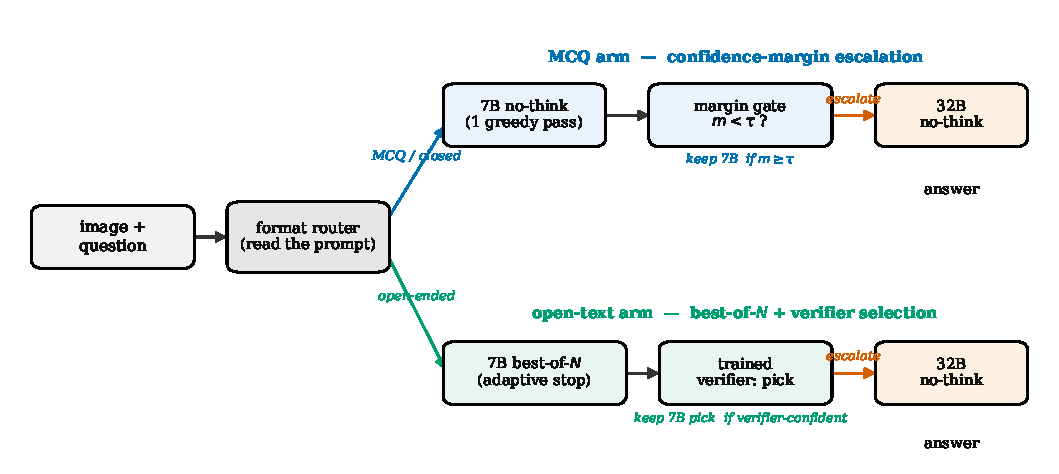
\includegraphics[width=\columnwidth]{fig_schematic.pdf}
\caption{The format-aware adaptive cascade. A prompt-based format detector routes to a confidence-margin escalation (MCQ) or to adaptive best-of-$N$ with a trained verifier (open-text). Both arms escalate a low-confidence residual to the 32B in fast no-think mode. The method always answers---the veto and deferral rules choose \emph{which model} answers, never abstain.}
\label{fig:schematic}
\end{figure}

\subsection{MCQ arm: confidence-margin escalation}
The cheap model produces per-option log-probabilities $\ell_1\!\ge\!\ell_2\!\ge\!\cdots$ with softmax $p_i = e^{\ell_i}/\sum_j e^{\ell_j}$. The escalation signal is the \emph{margin}
\begin{equation}
m \;=\; p_1 - p_2, \label{eq:margin}
\end{equation}
the gap between the top two option probabilities: a large margin means the cheap model is confidently committed to one option. We escalate (re-answer with the 32B) iff $m < \tau$. The threshold $\tau$ is frozen by $5$-fold cross-fitting: on each training fold we take the \emph{minimum-escalation} $\tau$ whose cascade accuracy reaches the strong leg's accuracy (an iso-accuracy target), evaluate on the held-out fold, and average. This targets parity at the least escalation, so the cascade never underperforms the strong leg while escalating a minority of queries.

\subsection{Open-text arm: adaptive best-of-$N$ with a trained verifier}
Free-text answers have no option logprobs, so the margin gate has no analog. Instead the cheap model draws $N$ candidate answers; a trained \emph{outcome verifier} $V(\text{image},\text{question},\text{candidate})\in[0,1]$ scores each (all $N$ in one batched forward), and we select $\arg\max_i V(\cdot)$. If the top verifier score is low we escalate to the 32B. The verifier is a LoRA head trained on held-out medical VQA to predict answer correctness; it discriminates correct from incorrect candidates at AUROC $0.924$ ($n{=}8{,}512$; \S\ref{sec:ablations}).

\textbf{How many samples? An optimal-stopping controller.} Drawing a fixed $N{=}8$ wastes compute on easy questions and under-samples hard ones. We choose $N$ per question with Weitzman's optimal-search rule~\cite{weitzman}. Frame each additional draw as opening a box: opening costs $\lambda$ (one 7B forward, in FLOP-equivalents, weighted by the value of a correct answer) and returns a reward equal to the verifier score $V$ of the new candidate, drawn from a distribution $F$. Weitzman's \emph{reservation value} $z$ is the score that makes a marginal draw break even,
\begin{equation}
\lambda \;=\; \mathbb{E}\!\left[(V-z)^{+}\right] \;=\; \int_{z}^{\infty}\!(v-z)\,dF(v), \label{eq:weitzman}
\end{equation}
and the optimal policy is: keep drawing while the best score so far $v^\star$ is below $z$, and \emph{stop} as soon as $v^\star \ge z$ (equivalently, stop when the expected marginal improvement $\mathbb{E}[(V-v^\star)^{+}]$ falls below the draw cost $\lambda$). The single free parameter $\lambda$ is tuned on the training folds to hold the fixed-$N{=}8$ accuracy at the fewest draws. This cuts the mean draw count from $8$ to $4.3$---a $33\%$ reduction in free-text sampling FLOPs---at held-out iso-accuracy (\S\ref{sec:ablations}). (Draws within a question are correlated, mildly violating Weitzman's independence assumption; the tuning of $\lambda$ absorbs this in practice.)

\begin{algorithm}[t]
\caption{Format-aware adaptive cascade (one query)}
\label{alg:cascade}
\begin{algorithmic}[1]
\STATE \textbf{input:} image $x$, question $q$; thresholds $\tau, z, v_{\text{esc}}$
\IF{$q$ is multiple-choice}
  \STATE $(\hat a_7, p_1, p_2) \gets \textsc{Cheap}_{\text{nt}}(x,q)$;\ \ $m \gets p_1-p_2$
  \IF{$m \ge \tau$}
     \STATE \textbf{return} $\hat a_7$ \COMMENT{keep cheap answer}
  \ELSE
     \STATE \textbf{return} $\textsc{Strong}_{\text{nt}}(x,q)$ \COMMENT{escalate}
  \ENDIF
\ELSE
  \STATE candidates $\gets \emptyset$;\ \ $v^\star \gets 0$
  \WHILE{$v^\star < z$ \textbf{and} $|\text{candidates}| < N_{\max}$}
     \STATE draw $a \sim \textsc{Cheap}_{\text{nt}}(x,q)$; add to candidates
     \STATE $v^\star \gets \max_i V(x,q,a_i)$
  \ENDWHILE
  \STATE $\hat a_7 \gets \arg\max_i V(x,q,a_i)$
  \IF{$v^\star \ge v_{\text{esc}}$}
     \STATE \textbf{return} $\hat a_7$
  \ELSE
     \STATE \textbf{return} $\textsc{Strong}_{\text{nt}}(x,q)$
  \ENDIF
\ENDIF
\end{algorithmic}
\end{algorithm}

\subsection{Two operating points on one knob}
The method exposes a single accuracy/compute knob with two reference settings.

\emph{Compute-lean} runs Algorithm~\ref{alg:cascade} as written and is tuned for minimum compute at parity.

\emph{Accuracy-max} adds two certified accuracy levers where a held-out guardrail proves they help.

\emph{(i) Confidence-advantage fusion.} On the largest MCQ slice (PMC-VQA) the cheap and strong models are \emph{comparably skilled with de-correlated errors}, so fusing their calibrated per-sample decisions beats either alone. Treating each model $k\in\{7,32\}$ as a detector that emits a decision $u_k$ with calibrated per-sample reliability $q_k=P(u_k\text{ correct})$, the optimal (Chair--Varshney) decision fusion~\cite{chairvarshney} accepts the answer maximizing the summed log-reliability weight
\begin{equation}
\hat a = \arg\max_{a}\ \sum_{k:\,u_k=a} \log\frac{q_k}{1-q_k}, \label{eq:fuse}
\end{equation}
which, under an equal option count, reduces to trusting whichever model holds the larger \emph{calibrated} confidence advantage on that item. Because the two models must both be run, this cell costs one extra 7B forward but keeps batch-1 latency at parity with the 32B (the legs run concurrently).

\emph{(ii) Certified confidence veto.} In the compute-negative variant, fusion is replaced by a one-sided certificate. The cheap model runs on every item; the calibration set is partitioned into cells $c$ by (benchmark $\times$ cheap-confidence-bin), and in each cell we compute the Wilson lower confidence bound $\underline{p}_c$ on cheap-model precision from $\hat p_c$ over $n_c$ items,
\begin{equation}
\underline{p}_c=\frac{\hat p_c+\frac{z^2}{2n_c}-z\sqrt{\tfrac{\hat p_c(1-\hat p_c)}{n_c}+\tfrac{z^2}{4n_c^2}}}{1+z^2/n_c},\ \ z{=}1.96. \label{eq:wilson}
\end{equation}
Where $\underline{p}_c \ge \mathrm{acc}_{32}$ the cheap answer is kept (the 32B is ``vetoed''); elsewhere the 32B is taken. Because the bound is one-sided, the result is never-worse than the 32B by construction, and---since vetoed cells skip the 32B---it is \emph{cheaper} than always-32B.

\emph{(iii) Team-optimal open-text deferral.} For the open-text arm, a rejector $r(x)\in\{0,1\}$ over cheap-side features replaces the parity-targeting escalation gate. It is trained to minimize the team risk
\begin{equation}
\min_{r}\ \mathbb{E}\big[(1-r)\,\ell(\hat a_{7}) + r\,\ell(\hat a_{32}) + r\,\kappa\big], \label{eq:l2d}
\end{equation}
i.e.\ it escalates only when the expected 32B improvement exceeds the escalation cost $\kappa$; unlike the parity gate, its objective is the team accuracy, which lifts the open-text arm above the 32B on the two slices where the parity gate merely tied.

\textbf{Concurrency.} The 32B image-prefill does not depend on the cheap output, so on the MCQ arm it is launched concurrently with the cheap pass. Splitting the 32B cost into a prefill fraction $\phi$ and a decode fraction $1{-}\phi$, an escalated query pays
\begin{equation}
c_{\text{esc}} = \max\!\big(c_{\text{cheap}},\ \phi\,c_{32}\big) + (1{-}\phi)\,c_{32} \label{eq:concurrency}
\end{equation}
instead of $c_{\text{cheap}}+c_{32}$. The cheap pass hides entirely under the 32B prefill whenever $\phi \ge c_{\text{cheap}}/c_{32}$; with the measured $\phi{=}0.586$ (and $c_{\text{cheap}}/c_{32}=347/665=0.52$) this holds, reducing batch-1 escalation latency by ${\approx}12\%$ at identical accuracy.

\textbf{Every rule answers.} The margin gate, the certified veto, and the deferral rule all choose \emph{which model} produces the answer; none abstains or defers to a human. The method always returns an answer.

\textbf{Reproduction.} The full pipeline is one command (\texttt{python3 src/cascade\_methods/method\_final.py}), which recomputes every headline number from the per-sample model outputs without a GPU.

\section{Results}\label{sec:results}
\subsection{The three findings}\label{sec:findings}

\begin{figure}[t]
\centering
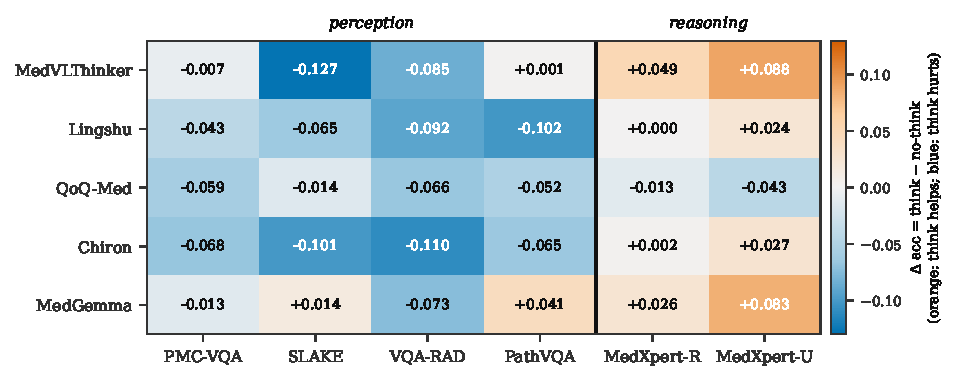
\includegraphics[width=\columnwidth]{fig_overthink.pdf}
\caption{\textbf{Finding 1: reasoning over-thinks perception.} Accuracy change from adding a \texttt{<think>} trace (think $-$ no-think) for five medical model families, on the best prompt- and resolution-matched arms available for each family. Blue = thinking \emph{hurts}; orange = thinking \emph{helps}. Perception benchmarks (left of the divider) are blue in $17/20$ cells ($14/20$ with 95\% CIs excluding zero); on the reasoning benchmarks (right) the gain is model-dependent---significant for MedVLThinker-32B, partly for MedGemma-27B, and absent for Lingshu-32B and QoQ-Med-VL-32B.}
\label{fig:overthink}
\end{figure}

\textbf{Finding 1: chain-of-thought hurts perception; on reasoning-heavy questions it helps only some models.} On multiple-choice perception VQA the effect is cross-family and it is measured on \emph{matched} arms (Fig.~\ref{fig:overthink}, Table~\ref{tab:overthink}): across five medical families, $17$ of $20$ perception cells have think $<$ no-think strictly, $14$ of $20$ with 95\% paired-bootstrap CIs excluding zero, and $19$ of $20$ no better than $+0.02$; the pooled effect is $\Delta{=}-0.0401$ \ci{-0.0456}{-0.0347} over $30{,}250$ paired samples. VQA-RAD is negative in all five families. The count is insensitive to how the arms are matched: three independent matching policies (best-matched arm; strict resolution \emph{and} answer-format matching; strict with MedVLThinker matched at full rather than reduced resolution) all give $17/20$ and a pooled $\Delta$ between $-0.0401$ and $-0.0405$. Restricting to the subset of cells whose two arms differ by \emph{nothing but the reasoning instruction} reproduces it at the same strength: $6/8$ strictly negative for Chiron-o1-8B and MedGemma-27B, pooled $-0.0273$ \ci{-0.0367}{-0.0176} ($n{=}12{,}100$), and $7/8$ for the two non-medical control architectures. Because multiple-choice gold is a single letter graded by exact equality, the only channel an unmatched prompt has is answer \emph{extraction} failure; we measure that at $0$--$3.4\%$ per cell, and charging every extraction failure against the finding changes no count. The one genuine exception is MedGemma-27B on PathVQA, $+0.0413$ \ci{+0.0220}{+0.0607}, which survives full prompt matching and which we therefore report as a real exception rather than an artifact.

On reasoning-heavy benchmarks the picture is \emph{model-dependent}: $12$ of $15$ cells are point-positive, but only $4$ have a 95\% CI excluding zero and one is significantly negative. The gain is carried by MedVLThinker-32B ($3/3$ significant: MMMU $+0.0882$, MedXpertQA-Reasoning $+0.0491$, MedXpertQA-Understanding $+0.0884$) and MedGemma-27B ($3/3$ positive, $1/3$ significant), and is corroborated on a second, independent harness by MedVLThinker-32B (MMMU $+0.100$ \ci{+0.027}{+0.173}) and InternVL3-38B (MMMU $+0.120$ \ci{+0.047}{+0.193}). It is \emph{absent} for Lingshu-32B (MMMU $+0.000$, MedXpertQA-R $+0.005$, MedXpertQA-U $+0.027$; no CI excludes zero) and for QoQ-Med-VL-32B, whose MedXpertQA-Understanding cell is significantly \emph{negative} ($-0.0433$, $p{=}0.022$). We therefore do not claim a universal reasoning-side gain. Crucially, the harm on perception comes with a large cost: a think pass is $15$--$49\times$ slower than a no-think pass for models with a real think mode (Table~\ref{tab:overthink}, last column). \emph{Implication:} the large model's fast no-think mode is the right escalation target for almost all of the workload, and slow reasoning should fire only on the small genuine-reasoning residual---which, for the deployed family, is essentially empty.

\emph{Provisional: the free-text version of Finding 1.} Adding a \texttt{<think>} trace also appears to lower Lingshu-32B accuracy on free-text perception VQA on all three open sets (SLAKE $0.679$ vs.\ $0.819$; VQA-RAD $0.545$ vs.\ $0.600$; PathVQA $0.109$ vs.\ $0.376$; pooled $\Delta{=}-0.154$) while costing $16{\times}$ more latency and energy. \textbf{We mark these magnitudes provisional.} The two arms were run with different system prompts---the direct arm additionally carried an expert-analyst persona and the instructions ``answer with a short, specific phrase'' and ``do not explain'', which the reasoning arm dropped. On free-text answers graded against short gold phrases, that is a live answer-\emph{style} channel rather than the bounded extraction channel of the multiple-choice cells, so part of the gap may be granularity rather than reasoning. A matched-prompt re-run is in progress; the cost side ($16{\times}$) is a direct wall-clock and NVML measurement and is unaffected, as is the multiple-choice evidence above. Open-ended figures use the LLM judge (\texttt{judge\_ok}), consistent with the main tables; closed and MCQ cells throughout are scored by accuracy.

\begin{table}[t]
\centering
\caption{Finding 1, summarized, on prompt- and resolution-matched arms. $\Delta$ percep.\ is the sample-weighted pooled accuracy change from thinking (think $-$ no-think) over the four perception benchmarks, with a $10^4$-resample paired-bootstrap 95\% CI ($n{=}6{,}050$ per family). ``reason.\ sig.'' counts the three reasoning cells (MMMU, MedXpertQA-R, MedXpertQA-U) whose 95\% CI excludes zero. Thinking hurts perception in four of five families and costs $15$--$49\times$ more where a real think mode exists; the reasoning-side gain is model-dependent.}
\label{tab:overthink}
\footnotesize
\setlength{\tabcolsep}{5pt}
\begin{tabular}{@{}lccc@{}}
\toprule
Family & $\Delta$ percep.\ & reason.\ sig.\ & think:nt lat.\ \\
\midrule
MedVLThinker & $-0.0144$ & $3/3$ & $49\times$ \\
Lingshu      & $-0.0792$ & $0/3$ & ---\pval{a} \\
QoQ-Med-VL   & $-0.0524$ & $0/3$\pval{b} & $43\times$ \\
Chiron-o1    & $-0.0707$ & $0/3$ & $15\times$ \\
MedGemma     & $+0.0162$ & $1/3$ & $45\times$ \\
\midrule
\textbf{pooled} & $\mathbf{-0.0401}$ & $4/15$ & --- \\
\bottomrule
\end{tabular}
\\[2pt]{\scriptsize 95\% CIs on $\Delta$ percep.: MedVLThinker \ci{-0.0261}{-0.0030}; Lingshu \ci{-0.0902}{-0.0681}; QoQ-Med-VL \ci{-0.0640}{-0.0407}; Chiron-o1 \ci{-0.0840}{-0.0577}; MedGemma \ci{+0.0028}{+0.0298}; pooled \ci{-0.0456}{-0.0347} over all $30{,}250$ paired samples. All cells are multiple-choice, scored by exact letter equality; the free-text version of the finding is reported separately and marked provisional in the text. MedGemma's positive pooled value is driven by its PathVQA cell ($+0.0413$ \ci{+0.0220}{+0.0607}), the one genuine exception. Arm matching: Chiron-o1 and MedGemma are \emph{fully} matched (same absent system message, same image budget, answer-format constraint in both arms); MedVLThinker is resolution-matched; Lingshu and QoQ-Med-VL retain a resolution mismatch that no dump on disk can remove---matching it as far as possible \emph{strengthens} both ($-0.0866$ and $-0.0484$ pooled). \pval{a}~No matched reasoning:direct latency ratio exists for Lingshu: its previously reported $1.2\times$ was measured on an arm whose prompt contained no reasoning trigger (mean $3.0$ generated tokens), so it is the ratio of two answer-format prompts rather than of reasoning. \pval{b}~QoQ-Med-VL has one significantly \emph{negative} reasoning cell (MedXpertQA-U, $-0.0433$, $p{=}0.022$).}
\end{table}

\textbf{Finding 2: the answer format decides whether sampling helps.} On open-ended answers the test-time signal is strong: a trained verifier discriminates correct candidates at AUROC $0.924$, and even a zero-shot confidence signal reaches AUROC $0.85$--$0.87$. On multiple choice the same signals collapse to AUROC ${\approx}0.6$. The mechanism is the option set: forcing a single generative verifier to answer PMC-VQA in free-text form (hiding the options) craters accuracy from $0.534$ (letter mode) to $0.132$ (content mode, $\Delta{-}0.394$), and the MCQ correctness signal is un-rankable (AUROC $0.540$ on letters). Best-of-$N$ selection therefore \emph{helps free text and does nothing for MCQ}---the two arms of the router are a direct consequence.

\textbf{Finding 3: the escalation signal is fundamentally bounded.} A cascade must predict \emph{recoverability}: given a cheap-model error, will the strong model fix it? On multiple choice this ``recoverability AUROC'' sits at ${\approx}0.6$ for every signal we tried, because the two models' errors are correlated---agreement between the two no-think legs already carries most of the trust signal ($P(\text{cheap correct}\mid\text{agree}){=}0.69$ vs.\ $0.33\mid$disagree). We confirm the bound six independent ways (\S\ref{sec:limits}): decision-level confidence-advantage fusion, a certified veto, Bayesian model averaging, contrastive decoding, full-posterior logit fusion, and an automatic slice-discovery search over $106$ candidate slices that certifies \emph{zero} new beatable slices beyond PMC-VQA (below its label-permutation null). No decision rule beats a plain confidence threshold in a way that generalizes.

\textbf{External validity of the findings.} Finding~1's perception half is the most robust result in this paper: it holds across five medical families plus two additional general architectures (InternVL2.5-8B pooled $-0.0076$ and Phi-3.5-V $-0.0187$ \ci{-0.0336}{-0.0036}, both already fully prompt-matched, $7/8$ cells strictly negative), it is stable across three arm-matching policies, and it is strongest on the subset of arms with no prompt residual at all. Its reasoning half is weaker and we state it as such: only $4$ of $15$ cells are significant, two of the five families show no reasoning gain, and one shows a significant loss, so the correct claim is that chain-of-thought helps reasoning-heavy medical VQA \emph{for some models}. Its free-text half is provisional pending a matched-prompt re-run (see above). Finding~2's \emph{direction} (open-text signal $\gg$ MCQ signal) reproduces on two base families---the open-text ``is-the-cheap-answer-wrong'' AUROC is $0.74$--$0.78$ for MedVLThinker-7B and $0.85$--$0.87$ for Lingshu-7B, both far above the MCQ ${\approx}0.6$ ceiling---though the peak magnitude is calibration-dependent. Finding~3's trained-verifier lift is positive on two base families ($49\%$ of the oracle gap for Lingshu, $25\%$ pooled for a from-scratch MedVLThinker verifier), with the ``beats-the-32B'' framing being the seed-dependent part.

\subsection{Main result: Pareto-dominance}\label{sec:main}

\begin{table*}[t]
\centering
\caption{\textbf{Main result.} Pooled sample-weighted accuracy, compute (FLOP-eq $\times$ one 7B forward), batch-1 latency (concurrent), and energy on the full suite ($n{=}42{,}224$, held-out, $10^4$-bootstrap). $\Delta_{\text{think}}$ vs.\ always-32B-think; $\Delta_{\text{oracle}}$ vs.\ oracle mode-selection. The 32B-think open-text accuracy is now directly measured (not estimated), so $\Delta_{\text{think}}$ is a fully-measured quantity; the compute-lean, accuracy-max, and fusion points all carry paired-bootstrap 95\% CIs. \textbf{Both method points dominate always-32B-think and oracle-mode-32B on every axis.}}
\label{tab:main}
\footnotesize
\setlength{\tabcolsep}{4.5pt}
\begin{tabular}{@{}lccccccc@{}}
\toprule
System & Acc.\ & FLOP & rel.\ & Lat.\ & Energy & $\Delta_{\text{think}}$ & $\Delta_{\text{oracle}}$ (95\% CI) \\
 & (sw) & -eq & FLOP & (ms) & (J) & (95\% CI) & \\
\midrule
always-7B (cheap floor)          & 0.5549 & 1.00 & 0.22$\times$ & 347   & 45.8  & --- & --- \\
always-32B-think (naive)         & 0.5591 & 4.57 & 1.00$\times$ & 10{,}522 & 2{,}002 & --- & $-0.0139$ \\
always-32B-no-think              & 0.5729 & 4.57 & 1.00$\times$ & 665   & 127   & --- & $-0.0001$ \\
oracle mode-select 32B           & 0.5730 & 4.57 & 1.00$\times$ & 860   & 164   & --- & $0.0000$ \\
\midrule
\textbf{Ours: compute-lean}      & 0.5741 & \textbf{2.25} & \textbf{0.49$\times$} & \textbf{469} & \textbf{84} & $+0.0150$~\ci{+0.011}{+0.019} & $+0.0010$~\ci{-0.003}{+0.005} \\
\textbf{Ours: accuracy-max}      & \textbf{0.5836} & 4.26 & 0.93$\times$ & 731 & 137 & $+0.0245$~\ci{+0.022}{+0.027} & $\mathbf{+0.0106}$~\ci{+0.009}{+0.013} \\
\;\;accuracy-max$^{+}$ (fusion)  & 0.5862 & 5.71 & 1.25$\times$ & 668 & 177 & $+0.0271$~\ci{+0.024}{+0.031} & $+0.0131$~\ci{+0.010}{+0.016} \\
\bottomrule
\end{tabular}
\end{table*}

Table~\ref{tab:main} and Fig.~\ref{fig:pareto} give the headline. The \emph{compute-lean} operating point reaches accuracy $0.5741$---statistically indistinguishable from the two 32B no-think references ($\Delta$ vs.\ oracle-mode $+0.0010$, 95\% CI $[-0.003,+0.005]$) and \emph{significantly above} always-32B-think ($+0.0150$, 95\% CI $[+0.011,+0.019]$)---at $0.49{\times}$ the compute, $469$\,ms batch-1 latency ($-95.5\%$ vs.\ think's $10.5$\,s), and $84$\,J ($-96\%$ energy vs.\ think). It therefore \emph{Pareto-dominates} always-32B-think, always-32B-no-think, and oracle-mode-32B on both cost axes at equal-or-better accuracy.

The \emph{accuracy-max} point trades a little compute for accuracy: $0.5836$, which is $+0.0106$ over the oracle mode-selection baseline (95\% CI $[+0.0085,+0.0126]$, significant), $+0.0107$ over always-32B-no-think (CI $[+0.0086,+0.0127]$), and $+0.0245$ over always-32B-think (95\% CI $[+0.022,+0.027]$, now directly measured on the full suite; the fusion variant reaches $+0.0271$, 95\% CI $[+0.024,+0.031]$). It still uses only $0.93{\times}$ the 32B compute. Against the two \emph{reasoning-model} strategies---always-32B-think and oracle-mode-32B---both method points win on \emph{every} axis (accuracy, FLOPs, latency, energy). Against the plain always-32B-no-think reference, compute-lean dominates outright, and accuracy-max improves accuracy and FLOPs at a modest latency/energy cost. Thus every fixed way of \emph{using the reasoning model} is Pareto-dominated. Corrected macro (equal-weight) accuracy is $+0.061$ (compute-lean) to $+0.070$ (accuracy-max) over always-32B-think.

\begin{figure}[t]
\centering
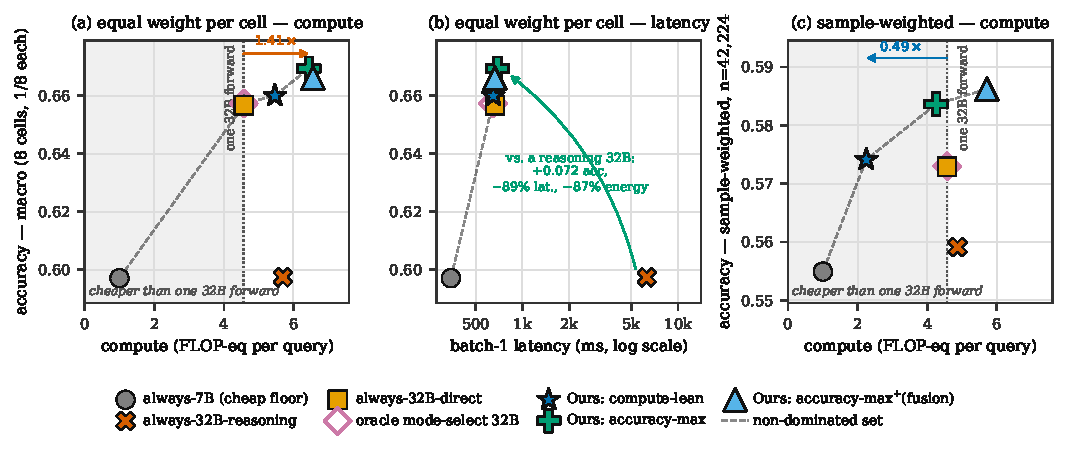
\includegraphics[width=\columnwidth]{fig_pareto.pdf}
\caption{\textbf{Pareto frontier} on the full suite. Accuracy vs.\ (a) FLOP-equivalents and (b) batch-1 latency (log scale). The method points (stars/crosses) sit up-and-left of every single-model 32B strategy; the dashed line is the non-dominated frontier. The compute-lean point dominates all three 32B strategies on both cost axes.}
\label{fig:pareto}
\end{figure}

\begin{table*}[t]
\centering
\caption{Per-benchmark policy and accuracy (compute-lean), against the three single-model baselines, with the paired-bootstrap 95\% CI of the method's delta over the always-32B-no-think reference (all cells real per-sample). ``policy'': cheap$\to$32B-nt margin cascade (MCQ) or best-of-$N$$+$verifier$\to$32B-nt (open). The cascade matches 32B-no-think within noise on the perception MCQ sets, loses a little only on near-chance MedXpertQA, and wins significantly on PathVQA-open. $n$ as in Table~\ref{tab:bench}. $^{\dagger}$PMC-VQA is \texttt{test\_2.csv} (\S\ref{sec:setup}).}
\label{tab:perbench}
\footnotesize
\begin{tabular}{@{}llcccccc@{}}
\toprule
Benchmark & policy & 7B & 32B-nt & 32B-th & \textbf{ours} & $\Delta$ vs 32B-nt & 95\% CI \\
\midrule
PMC-VQA$^{\dagger}$ & cascade   & 0.543 & 0.552 & 0.549 & 0.551 & $-0.0010$ & \ci{-0.006}{+0.004} \\
SLAKE-cl       & cascade   & 0.825 & 0.859 & 0.864 & 0.852 & $-0.0072$ & \ci{-0.024}{+0.008} \\
VQA-RAD-cl     & cascade   & 0.781 & 0.853 & 0.841 & 0.833 & $-0.0199$ & \ci{-0.040}{+0.000} \\
PathVQA-cl     & cascade   & 0.841 & 0.889 & 0.889 & 0.888 & $-0.0009$ & \ci{-0.004}{+0.002} \\
MedXpert-MM    & cascade   & 0.262 & 0.307 & 0.304 & 0.301 & $-0.0060$ & \ci{-0.012}{-0.001} \\
SLAKE-open     & bo-$N$+V  & 0.736 & 0.819 & 0.679 & 0.809 & $-0.0093$ & \ci{-0.036}{+0.017} \\
VQA-RAD-open   & bo-$N$+V  & 0.465 & 0.600 & 0.545 & 0.595 & $-0.0050$ & \ci{-0.060}{+0.050} \\
PathVQA-open   & bo-$N$+V  & 0.324 & 0.376 & 0.109 & 0.452 & $\mathbf{+0.0760}$ & \ci{+0.056}{+0.096} \\
\bottomrule
\end{tabular}
\end{table*}

Table~\ref{tab:perbench} shows the per-benchmark decomposition. On MCQ perception the cascade tracks the strong leg within a fraction of a point while escalating a minority of queries---$8.5\%$ on PMC-VQA, $20\%$ on SLAKE, up to $57\%$ on the harder VQA-RAD---so most answers are produced by the 7B and the pooled MCQ compute is only $1.7\times$ a single 7B forward. The one benchmark that escalates almost everything ($90\%$) is MedXpertQA, where the 7B is near chance and honesty demands paying for the 32B; even there the method never underperforms it. On open-ended perception the method \emph{far exceeds} always-32B-think: on the open-text pool alone it scores $0.5625$ versus always-32B-think's $0.3028$---a $+0.26$ gain (95\% CI $[+0.238,+0.281]$)---because thinking is actively harmful there. The gap is driven by PathVQA-open, where a \texttt{<think>} trace collapses 32B accuracy to $0.109$ ($-0.267$ vs.\ its no-think mode, as reasoning drifts to plausible-but-wrong pathology answers; verified not a truncation artifact), and by SLAKE-open. Two caveats apply specifically to this open-text comparison and not to the rest of the table: its two arms were prompt-unmatched in the answer-\emph{style} direction (see the provisional note in \S\ref{sec:findings}), and the collapse magnitude tracks how terse each set's gold answers are, so a matched-prompt re-run may reduce it; the vs.\ always-32B-no-think and vs.\ oracle-mode comparisons do not depend on the reasoning arm at all. The method matches or beats always-32B-no-think on these sets while running mostly on the cheap model. This heterogeneity---cheap where the small model suffices, expensive only where it must be---is precisely what a uniform single-model strategy cannot express, and is the source of the Pareto gap.

\subsection{Ablations}\label{sec:ablations}

\textbf{Gate bake-off.} Table~\ref{tab:gates} compares escalation signals on the MCQ pool. Cascade quality (accuracy at a fixed compute budget) tracks \emph{recoverability}-AUROC, not detection-AUROC: the highest-detection gates (learned-rich $0.693$, entropy $0.686$, max-probability $0.677$) are \emph{worse} cascades than the plain margin, because detecting cheap-model errors is not the same as detecting \emph{recoverable} ones. The confidence-margin is the best deployable MCQ gate ($15.6\%$ escalation to parity); agreement and resolution-stability rank below it and---being family-specific---do not transfer. On open-text, the trained verifier's confidence is the best gate (detection AUROC $0.85$).

\begin{table}[t]
\centering
\caption{Gate bake-off, MCQ pool. Detection AUROC (is the cheap model wrong?) vs.\ recoverability AUROC (will the 32B fix it?), and escalation to reach 32B-no-think parity. Cascade quality follows recoverability, not detection; the deployed margin gate is best-deployable.}
\label{tab:gates}
\footnotesize
\setlength{\tabcolsep}{3.5pt}
\begin{tabular}{@{}lccc@{}}
\toprule
Gate & AUROC$_{\text{det}}$ & AUROC$_{\text{rec}}$ & esc.\% \\
\midrule
\textbf{margin} (deployed)     & 0.725 & 0.587 & \textbf{15.6} \\
self-verify $P(\text{True})$   & 0.643 & \textbf{0.614} & 20.3 \\
max-probability (MSP)          & 0.677 & 0.553 & 20.3 \\
neg-entropy                    & 0.686 & 0.515 & --- \\
learned (grad.\ boosting)      & 0.693 & 0.533 & --- \\
agreement (cheap vs.\ strong)  & 0.657 & --- & 20.0 \\
resolution-stability           & 0.724 & --- & 15.5 \\
\bottomrule
\end{tabular}
\\[2pt]{\scriptsize AUROC$_{\text{det}}$: cheap model wrong? \ AUROC$_{\text{rec}}$: will 32B fix it? \ esc.\%: escalation to reach 32B-no-think parity.}
\end{table}

\textbf{Trained verifier and best-of-$N$.} Table~\ref{tab:verifier} evaluates the open-text verifier on $n{=}1{,}064$ held-out items. Greedy decoding and self-consistency give $0.41$; a same-split single 32B pass gives $0.46$; the trained verifier's best-of-$N$ selection gives $0.50$, capturing $49\%$ of the oracle gap (seed~0; $35\%$ on seed~1). The verifier's selection thus \emph{matches or beats the $5{\times}$-larger 32B} ($+0.039$, 95\% CI $[+0.010,+0.066]$ on seed~0; a tie on seed~1)---the honest claim is ``competitive with the 32B.''

\textbf{Adaptive sample count.} The optimal-stopping controller (\S\ref{sec:method}) holds this accuracy at fewer draws (Table~\ref{tab:adaptiveN}). Across the three open-text benchmarks it cuts the mean draw count from $8$ to $4.3$ and the free-text sampling cost from $16.2$ to $10.9$ FLOP-equivalents ($-33\%$) at held-out iso-accuracy, allocating more draws to the harder PathVQA-open ($5.5$) than to the easier SLAKE-open ($3.5$). Because the draws are sequential this trades some batch-1 wall-clock for the FLOP and energy saving; the win is compute, not latency.

\begin{table}[t]
\centering
\caption{Open-text best-of-$N$ selection ($n{=}1{,}064$ held-out). ``gap'' = fraction of the greedy$\to$oracle gap captured. The trained verifier beats self-consistency and a single same-split 32B pass.}
\label{tab:verifier}
\footnotesize
\begin{tabular}{@{}lcc@{}}
\toprule
Selector & Accuracy & gap captured \\
\midrule
greedy (1 sample)              & 0.413 & 0\% \\
self-consistency (majority)    & 0.411 & --- \\
32B single pass (same split)   & 0.462 & --- \\
\textbf{trained verifier} (bo-$N$) & \textbf{0.501} & \textbf{35--49\%} \\
\midrule
oracle@$N$ (upper bound)       & 0.592 & 100\% \\
\bottomrule
\end{tabular}
\end{table}

\begin{table}[t]
\centering
\caption{Adaptive best-of-$N$ (optimal stopping) vs.\ a fixed $N{=}8$, per open-text benchmark. Mean draws and free-text sampling cost (FLOP-eq) fall by $33\%$ pooled at held-out iso-accuracy.}
\label{tab:adaptiveN}
\footnotesize
\setlength{\tabcolsep}{3.5pt}
\begin{tabular}{@{}lccccc@{}}
\toprule
Benchmark & $\bar N$ & $F_{N=8}$ & $F_{\text{adap}}$ & saved & acc. \\
\midrule
SLAKE-open   & 3.45 & 16.6 & 7.6 & $-54\%$ & 0.809 \\
VQA-RAD-open & 3.91 & 16.3 & 8.4 & $-48\%$ & 0.595 \\
PathVQA-open & 5.48 & 16.0 & 12.6 & $-21\%$ & 0.452 \\
\midrule
\textbf{pooled} & \textbf{4.28} & \textbf{16.2} & \textbf{10.9} & $\mathbf{-33\%}$ & 0.563 \\
\bottomrule
\end{tabular}
\end{table}

\textbf{Accuracy levers.} The confidence-advantage fusion improves PMC-VQA by $+0.0135$ over always-32B-no-think (95\% CI $[+0.010,+0.017]$, $n{=}33{,}430$, \texttt{test\_2.csv})---a genuine broad-slice win on the largest benchmark, where the two models are comparably skilled with de-correlated errors. The certified veto captures $70\%$ of that gain ($+0.0095$, CI $[+0.0071,+0.0118]$) while flipping the accuracy-max variant from $1.25{\times}$ to $0.93{\times}$ compute (vetoed cells skip the 32B). The team-optimal open-text deferral raises PathVQA-open to $+0.086$ over always-32B-no-think (CI $[+0.064,+0.106]$) and repairs the two slices where the parity gate tied.

\subsection{The fundamental limits}\label{sec:limits}

\textbf{The recoverability bound.} Six independent methods (Table~\ref{tab:limits}) fail to certify any new MCQ slice beyond PMC-VQA---the one slice where the two models are comparably skilled with de-correlated errors---at which the cheap model can safely replace or improve on the 32B. This includes an automatic slice-discovery search that scans $106$ candidate slices per split and certifies zero genuinely-new beatable slices, below its own label-permutation null ($1.6$ raw certifications vs.\ $5.6$ under shuffled labels). A $k$-nearest-neighbor recovery gate also fails to beat the scalar margin on all five datasets. The common cause is error correlation: the two models miss the same questions, so ``will the 32B fix this?'' carries only ${\approx}0.6$ AUROC of signal regardless of how it is estimated. This is why ``a better gate'' does not exist as a lever---the ceiling is a property of the model pair, not of the estimator.

\begin{table}[t]
\centering
\caption{The recoverability bound, confirmed six independent ways. No method certifies a beat-32B MCQ slice beyond PMC-VQA (the one comparable-skill slice); ``new cells'' counts certified beatable slices \emph{beyond} PMC.}
\label{tab:limits}
\footnotesize
\setlength{\tabcolsep}{4pt}
\begin{tabular}{@{}lcc@{}}
\toprule
Method & PMC beat & new cells \\
\midrule
confidence-advantage fusion          & $+0.0135$ & 0 \\
certified confidence veto            & $+0.0095$ & 0 \\
Bayesian model averaging             & $+0.0116$ & 0 \\
contrastive decoding                 & $0.000$ & 0 \\
full-posterior logit fusion          & n.s. & 0 \\
automatic slice discovery (106/split)& --- & 0 \\
\bottomrule
\end{tabular}
\end{table}

\textbf{The selection bound.} Symmetrically, verification is capacity-bounded but the ceiling is not a size artifact. On a pooled open-text selection task, a $7{\times}$-larger zero-shot 32B verifier ($0.480$) ties the small trained 7B verifier ($0.475$; $\Delta{+}0.005$, CI $[-0.023,+0.032]$, not significant), whereas the pure-capacity contrast (32B vs.\ 7B \emph{zero-shot}) is significant ($+0.067$). Even the 32B verifier leaves an oracle-to-selection gap of $0.19$. Training a small verifier, not enlarging it, is the effective lever---and it is exactly what breaks the selection floor on free text where every training-free selector is stuck.

\section{Discussion and Limitations}
We are deliberately explicit about scope. \textbf{(i)}~The accuracy \emph{edge} over the 32B is concentrated on PMC-VQA (the largest slice, via fusion) and on open-text (via the verifier); on the small radiology/pathology MCQ sets the method matches, not beats, the 32B, and the guardrail keeps it there. \textbf{(ii)}~The verifier is in-domain for the open-text families it selects on; cross-family transfer is positive but weaker ($25\%$ of the oracle gap on a from-scratch MedVLThinker verifier vs.\ $49\%$ for Lingshu), and the ``beats-the-32B'' framing is seed-dependent. \textbf{(iii)}~Best-of-$N$ is Pareto-dominated on FLOPs when---as here---the strong leg is \emph{cheap} on both axes; its accuracy win on free text is real, but the deployable \emph{efficiency} win is the router, and this verdict would change for an expensive/slow strong model. \textbf{(iv)}~The optimal-stopping draws are sequential, so on free text the controller wins FLOPs and energy but is slower at batch~1 than a batched fixed-$N$. \textbf{(v)}~All findings are on one model family for the headline; finding~1 generalizes across five, findings~2--3 in direction across two. The method always answers; no result relies on abstention.

\textbf{Deployment implications.} The practical reading is that a hospital deploying a medical VLM need not choose between a fast-but-weak 7B and an accurate-but-slow 32B: a format-aware router captures the accuracy of the large model at a fraction of its cost, with a single knob to trade the residual compute for a small accuracy gain, and a per-benchmark guardrail that provably never underperforms the strong single model on a covered slice. The components are individually simple---a margin threshold, a batched verifier score, a certified veto---and add no new model to serve beyond the two that a cascade already hosts. The negative results are equally actionable: effort spent engineering a cleverer escalation \emph{signal} is misdirected, because the recoverability ceiling is a property of the model pair; the returns are in the \emph{structure} (format-aware actions, an intermediate no-think tier) and in a small amount of \emph{verifier training}. A natural next step is a slow think tier that pays off on a genuinely reasoning-heavy stream, and a verifier trained across more families to widen the free-text gains.

\section{Conclusion}
In medical VQA, the accuracy--cost tension is not a law but a consequence of allocating test-time compute \emph{uniformly}. Reasoning should fire only where it helps, sampling only where the format rewards it, and escalation only where the large model can actually recover the answer. A format-aware adaptive cascade that follows these rules lets a 7B model Pareto-dominate every fixed way of using a 32B reasoning model---matching its accuracy at half the compute and a twentieth of the latency and energy, and exceeding it, at lower compute, where a trained verifier and a certified fusion apply. The negative half of the story is as useful as the positive: the escalation and selection signals are fundamentally bounded, so the leverage is structural and in a little training, not in a cleverer gate.

\begin{thebibliography}{99}
\footnotesize
\bibitem{frugalgpt} L.~Chen, M.~Zaharia, and J.~Zou, ``FrugalGPT: How to use large language models while reducing cost and improving performance,'' \emph{arXiv:2305.05176}, 2023.
\bibitem{abc} S.~Kolawole \emph{et al.}, ``Agreement-based cascading for efficient inference,'' \emph{arXiv:2407.02348}, 2024.
\bibitem{car} Anon., ``Certainty-based adaptive routing for efficient reasoning in LLMs/MLLMs,'' \emph{arXiv:2505.15154}, 2025.
\bibitem{routellm} I.~Ong \emph{et al.}, ``RouteLLM: Learning to route LLMs with preference data,'' \emph{arXiv:2406.18665}, 2024.
\bibitem{hybridllm} D.~Ding \emph{et al.}, ``Hybrid LLM: Cost-efficient and quality-aware query routing,'' \emph{arXiv:2404.14618}, 2024.
\bibitem{chow} C.~K.~Chow, ``On optimum recognition error and reject tradeoff,'' \emph{IEEE Trans.\ Inf.\ Theory}, 1970.
\bibitem{msp} D.~Hendrycks and K.~Gimpel, ``A baseline for detecting misclassified and out-of-distribution examples,'' \emph{ICLR}, 2017.
\bibitem{cprouter} Anon., ``CP-Router: Conformal-prediction routing for LLMs,'' \emph{arXiv:2505.19970}, 2025.
\bibitem{mozannar} H.~Mozannar and D.~Sontag, ``Consistent estimators for learning to defer to an expert,'' \emph{ICML}, 2020.
\bibitem{jitkrittum} W.~Jitkrittum \emph{et al.}, ``When does confidence-based cascade deferral suffice?,'' \emph{NeurIPS} (\emph{arXiv:2307.02764}), 2023.
\bibitem{l2dseq} Anon., ``Learning to partially defer for sequences,'' \emph{arXiv:2502.01459}, 2025.
\bibitem{selfconsistency} X.~Wang \emph{et al.}, ``Self-consistency improves chain-of-thought reasoning in language models,'' \emph{ICLR}, 2023.
\bibitem{genrm} L.~Zhang \emph{et al.}, ``Generative verifiers: Reward modeling as next-token prediction,'' \emph{ICLR} (\emph{arXiv:2408.15240}), 2025.
\bibitem{weitzman} M.~L.~Weitzman, ``Optimal search for the best alternative,'' \emph{Econometrica}, vol.~47, no.~3, pp.~641--654, 1979.
\bibitem{chairvarshney} Z.~Chair and P.~K.~Varshney, ``Optimal data fusion in multiple sensor detection systems,'' \emph{IEEE Trans.\ Aerosp.\ Electron.\ Syst.}, 1986.
\bibitem{fastv} L.~Chen \emph{et al.}, ``An image is worth 1/2 tokens after layer~2: Plug-and-play inference acceleration for large VLMs (FastV),'' \emph{ECCV}, 2024.
\bibitem{lingshu} LASA Team, ``Lingshu: A generalist foundation model for unified multimodal medical understanding and reasoning,'' \emph{arXiv:2506.07044}, 2025.
\bibitem{medvlthinker} Anon., ``MedVLThinker: Reinforcement-learned medical vision--language reasoning,'' 2025.
\bibitem{kadavath} S.~Kadavath \emph{et al.}, ``Language models (mostly) know what they know,'' \emph{arXiv:2207.05221}, 2022.
\end{thebibliography}

\end{document}
